\section{Operations: RDM in Practice}
{
    \setbeamertemplate{background canvas}{
        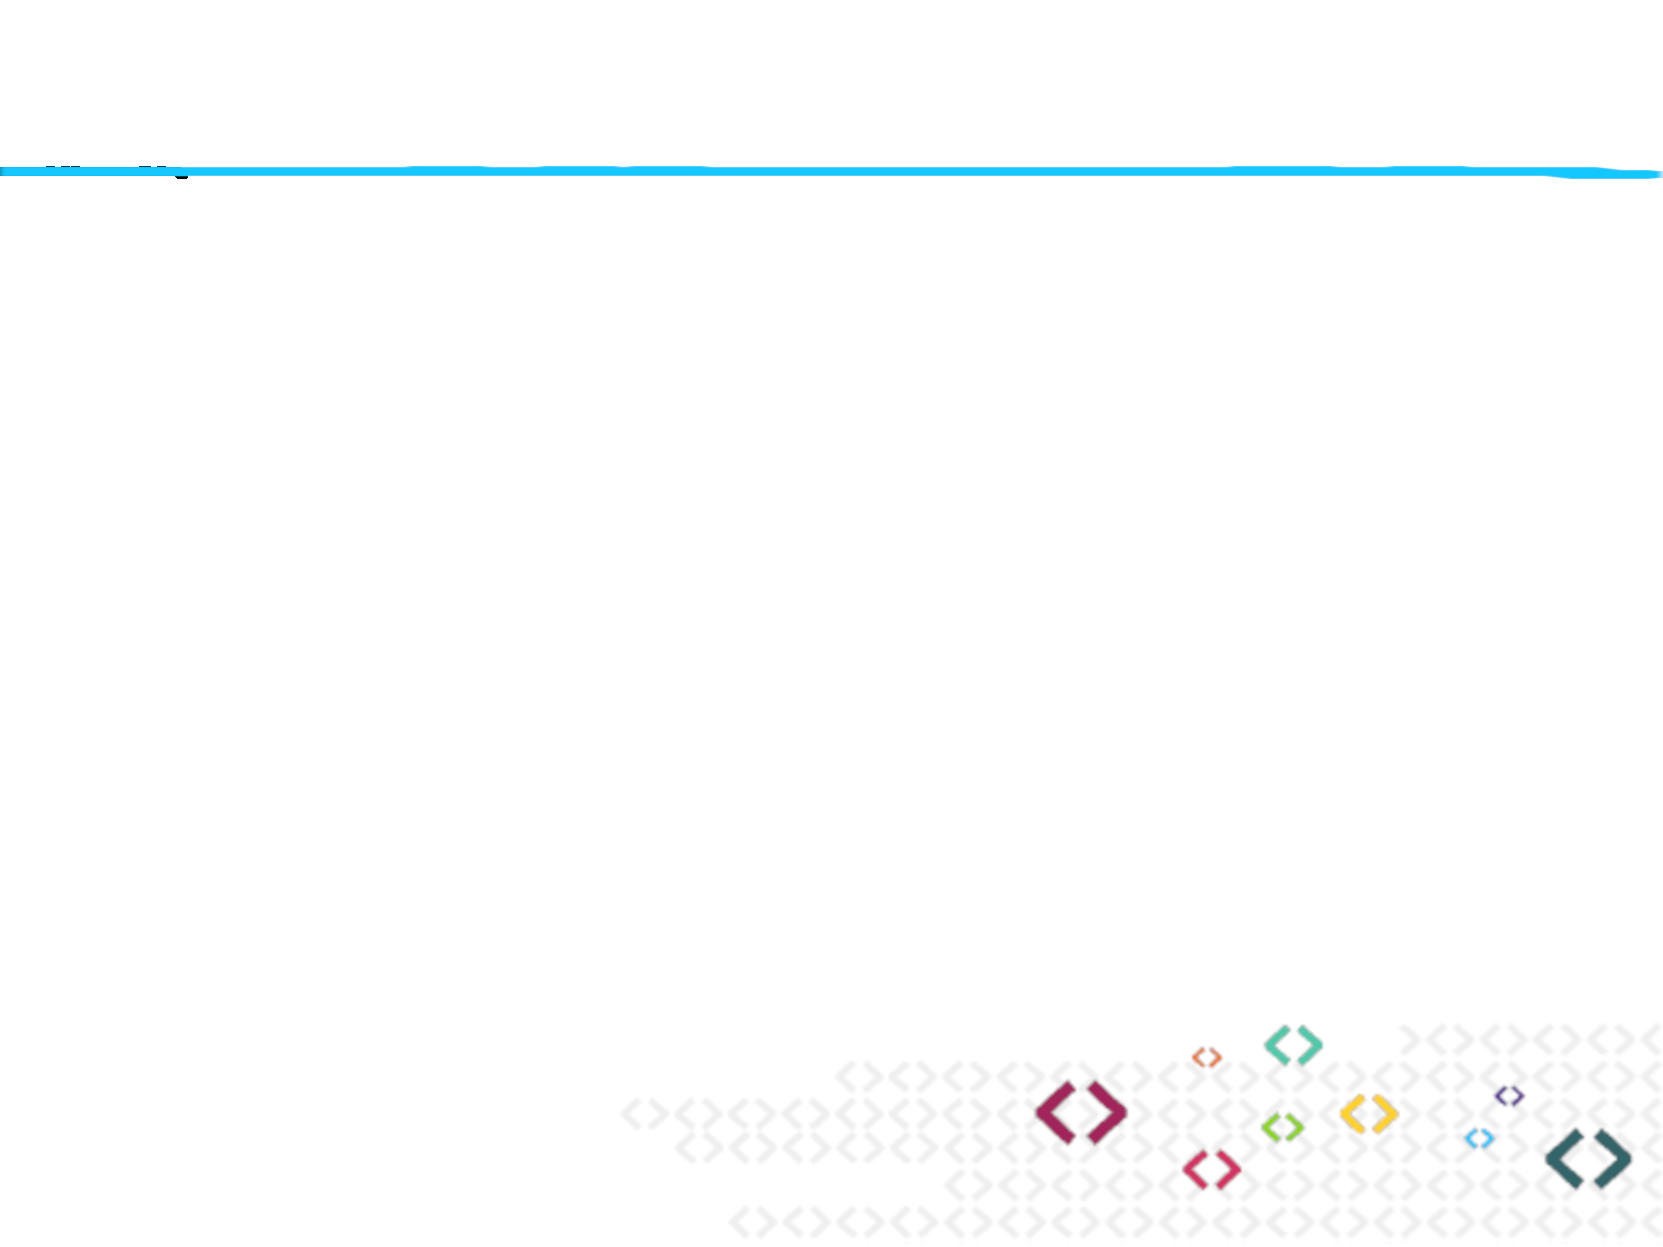
\includegraphics[width=\paperwidth,height=\paperheight]{figs/background_white.png}
    }
    \begin{frame}[plain]{Day 1 - Part 3: RDM in Research Operations}
        %% %% \frametitle{12:15 - 13:00}
        \begin{block}{Module 3 Goal}
            A plan is useless without action. We will learn to integrate RDM (ELNs, Git, Pipelines) into our \textbf{daily research operations}.
        \end{block}
       %% \begin{center}
       %%     \includegraphics[width=0.6\textwidth]{example-image-a}
       %%     \captionof{figure}{From blueprint (DMP) to construction (Operation).}
       %% \end{center}
    \end{frame}
}

\begin{frame}{Learning Objectives (3.1)}
    \begin{itemize}
        \item \textbf{List} the mandatory data records (e.g., metadata, raw data, scripts) required for project closure.
        \item \textbf{Identify} the mandatory metadata fields (e.g., sample ID, instrument ID) to be logged in an \textbf{ELN} upon acquisition.
    \end{itemize}
\end{frame}

\begin{frame}{Theory: The "Project Closure" Package}{Module 3.1: List}
    When your project ends, you must archive a "research package" that ensures Reusability and meets DFG's 10-year rule.
    
    \begin{block}{Mandatory Records for Archiving}
        \begin{itemize}
            \item \textbf{1. Raw Data:} The original, unaltered files from the instrument.
            \pause
            \item \textbf{2. Processed Data:} The final, clean data used for figures.
            \pause
            \item \textbf{3. Metadata:} The `README` or `metadata.xml` that describes everything.
            \pause
            \item \textbf{4. Scripts:} The code (e.g., Python, R, Matlab) used to get from Raw to Processed.
            \pause
            \item \textbf{5. Documentation:} The ELN export, codebook, or lab journal.
        \end{itemize}
    \end{block}
\end{frame}

\begin{frame}{Theory: The ELN at Acquisition}{Module 3.1: Identify}
    To build that archive, you must capture metadata \emph{at the moment of acquisition} in your \textbf{Electronic Lab Notebook (ELN)}.
    
    %% \begin{columns}
        %% \column{.5\textwidth}
        %% \includegraphics[width=\textwidth]{example-image-b}
        
        %% \column{.5\textwidth}
        \begin{block}{Mandatory ELN Fields \cite{zb_med-informationszentrum_lebenswissenschaften_electronic_2021}}
            Your ELN template for a new experiment should \textbf{force} you to enter:
            \begin{itemize}
                \item `\texttt{experiment\_ID}`, `\texttt{operator\_name}`
                \item `\texttt{date\_time}` (timestamp), `\texttt{instrument\_ID}`
                \item `\texttt{sample\_ID(s)}`, `\texttt{project\_name}`
                \item `\texttt{hypothesis}` (Why are you doing this?)
            \end{itemize}
        \end{block}
    %% \end{columns}
    \pause
    If you don't record this \emph{now}, it is lost forever. This is the core of operational data integrity.
\end{frame}

\begin{frame}{Interactive: Design Your ELN Template}{Module 3.1: Practice}
    \begin{block}{Activity: Your ELN Template (10 min)}
        \textbf{Task:} You are setting up a new ELN (e.g., \href{https://demo-kadi4mat.iam.kit.edu}{https://demo-kadi4mat.iam.kit.edu}). You are creating a template for a "standard experiment" in your field.
        \pause
        \textbf{Brainstorm:}
        \begin{itemize}
            \item \textbf{List} 5-10 \textbf{mandatory metadata fields} you must capture.
            \item \textbf{Identify} the \textit{one} field that is most often forgotten, but causes the most problems later.
        \end{itemize}
        \pause
        \textbf{Goal:} \textbf{Identify} mandatory fields for your ELN.
        \href{https://demo-kadi4mat.iam.kit.edu/templates/8}{$\therefore$}
    \end{block}
\end{frame}

\begin{frame}{Learning Objectives (3.2)}
    \begin{itemize}
        \item \textbf{Summarise} the differences in data access controls and their impact on operational security.
        \item \textbf{Illustrate} how connecting an \textbf{Instrument Registry} to the ELN automatically fulfils 'F' and 'I'.
    \end{itemize}
\end{frame}

\begin{frame}{Theory: Access Controls in Operation}{Module 3.2: Summarise}
    Access controls are not just for publishing. They are for \emph{operational security} during the project.
    
    \begin{itemize}
        \item \textbf{Problem:} Your "in-progress" data is often your most sensitive asset.
        \pause
        \item \textbf{Risk 1 (Too Open):} Data on a shared drive with no access control. A student from another group accidentally deletes it. (Integrity failure!)
        \pause
        \item \textbf{Risk 2 (Too Closed):} Data on your personal laptop. If you get sick, your team cannot continue working. (Operational failure!)
        \pause
        \item \textbf{Solution:} Use \textbf{role-based access}.
        \begin{itemize}
            \item `Project\_Leader`: Read/Write
            \item `PhD\_Student`: Read/Write
            \item `Master\_Student`: Read-Only (on raw data)
            \item `External\_Collaborator`: Read-Only (on processed data)
        \end{itemize}
    \end{itemize}
\end{frame}

\begin{frame}{Theory: The Instrument Registry}{Module 3.2: Illustrate}
    %% \begin{center}
    %%     \includegraphics[width=0.8\textwidth]{example-image-c}
    %%     \captionof{figure}{Manual vs. Automated ELN Entry}
    %% \end{center}
    
    \begin{columns}
        \column{.4\textwidth}
            \begin{block}{Manual Way (Low 'I')}
            \textbf{ELN Field:} `instrument\_name` \\
            \textbf{You type:} "The new microscope in room 205" \\
            \pause
            \textbf{Problem:} This is free-text. It's not machine-readable. It's not interoperable. \\
        \end{block}
        
        \column{.6\textwidth}
        \begin{block}{Automated Way (High 'I')}
            An \textbf{Instrument Registry} is a database of all lab equipment. \\
            \pause
            \textbf{ELN Field:} `instrument\_ID` \\
            \textbf{You select:} `HMC-KIT-Microscope-047` \\
            \pause
            \textbf{Result:} Your data is now \emph{linked} to that instrument's entire history (calibration, model, etc.). \\
            This is \textbf{Interoperability ('I')} and \textbf{Findability ('F')}!
        \end{block}
    \end{columns}
\end{frame}

\begin{frame}{Interactive: Your Security Workflow}{Module 3.2: Practice}
    \begin{block}{Discussion (10 min)}
        \textbf{Task:} \textbf{Summarise} the access controls on your current project's "in-progress" data.
        \pause
        \begin{itemize}
            \item Who has access?
            \item Is it too open or too closed?
            \item How does this impact your operational security?
        \end{itemize}
        \pause
        \textbf{Illustration:}
        \begin{itemize}
            \item \textbf{Illustrate} (by drawing a diagram) how connecting your lab's instrument list (even a simple Excel file) to your ELN would improve your data's 'I' and 'R' value.
        \end{itemize}
    \end{block}
    ex. \href{https://sms.atmohub.kit.edu}{Sensor Management System} delivers PIDs like :
    https://hdl.handle.net/21.11157/b88fe935-2072-4106-8aca-f008e2feab48
\end{frame}

\begin{frame}{Learning Objectives (3.3)}
    \begin{itemize}
        \item \textbf{Execute} the process of version control (e.g., using Git) on analysis scripts, ensuring \textbf{traceability}.
        \item \textbf{Configure} a \textbf{message broker} (e.g., Kafka) to route data streams from an instrument.
    \end{itemize}
\end{frame}

\begin{frame}{Theory: Version Control for Traceability}{Module 3.3: Execute}
    \begin{columns}
        \column{.36\textwidth}
        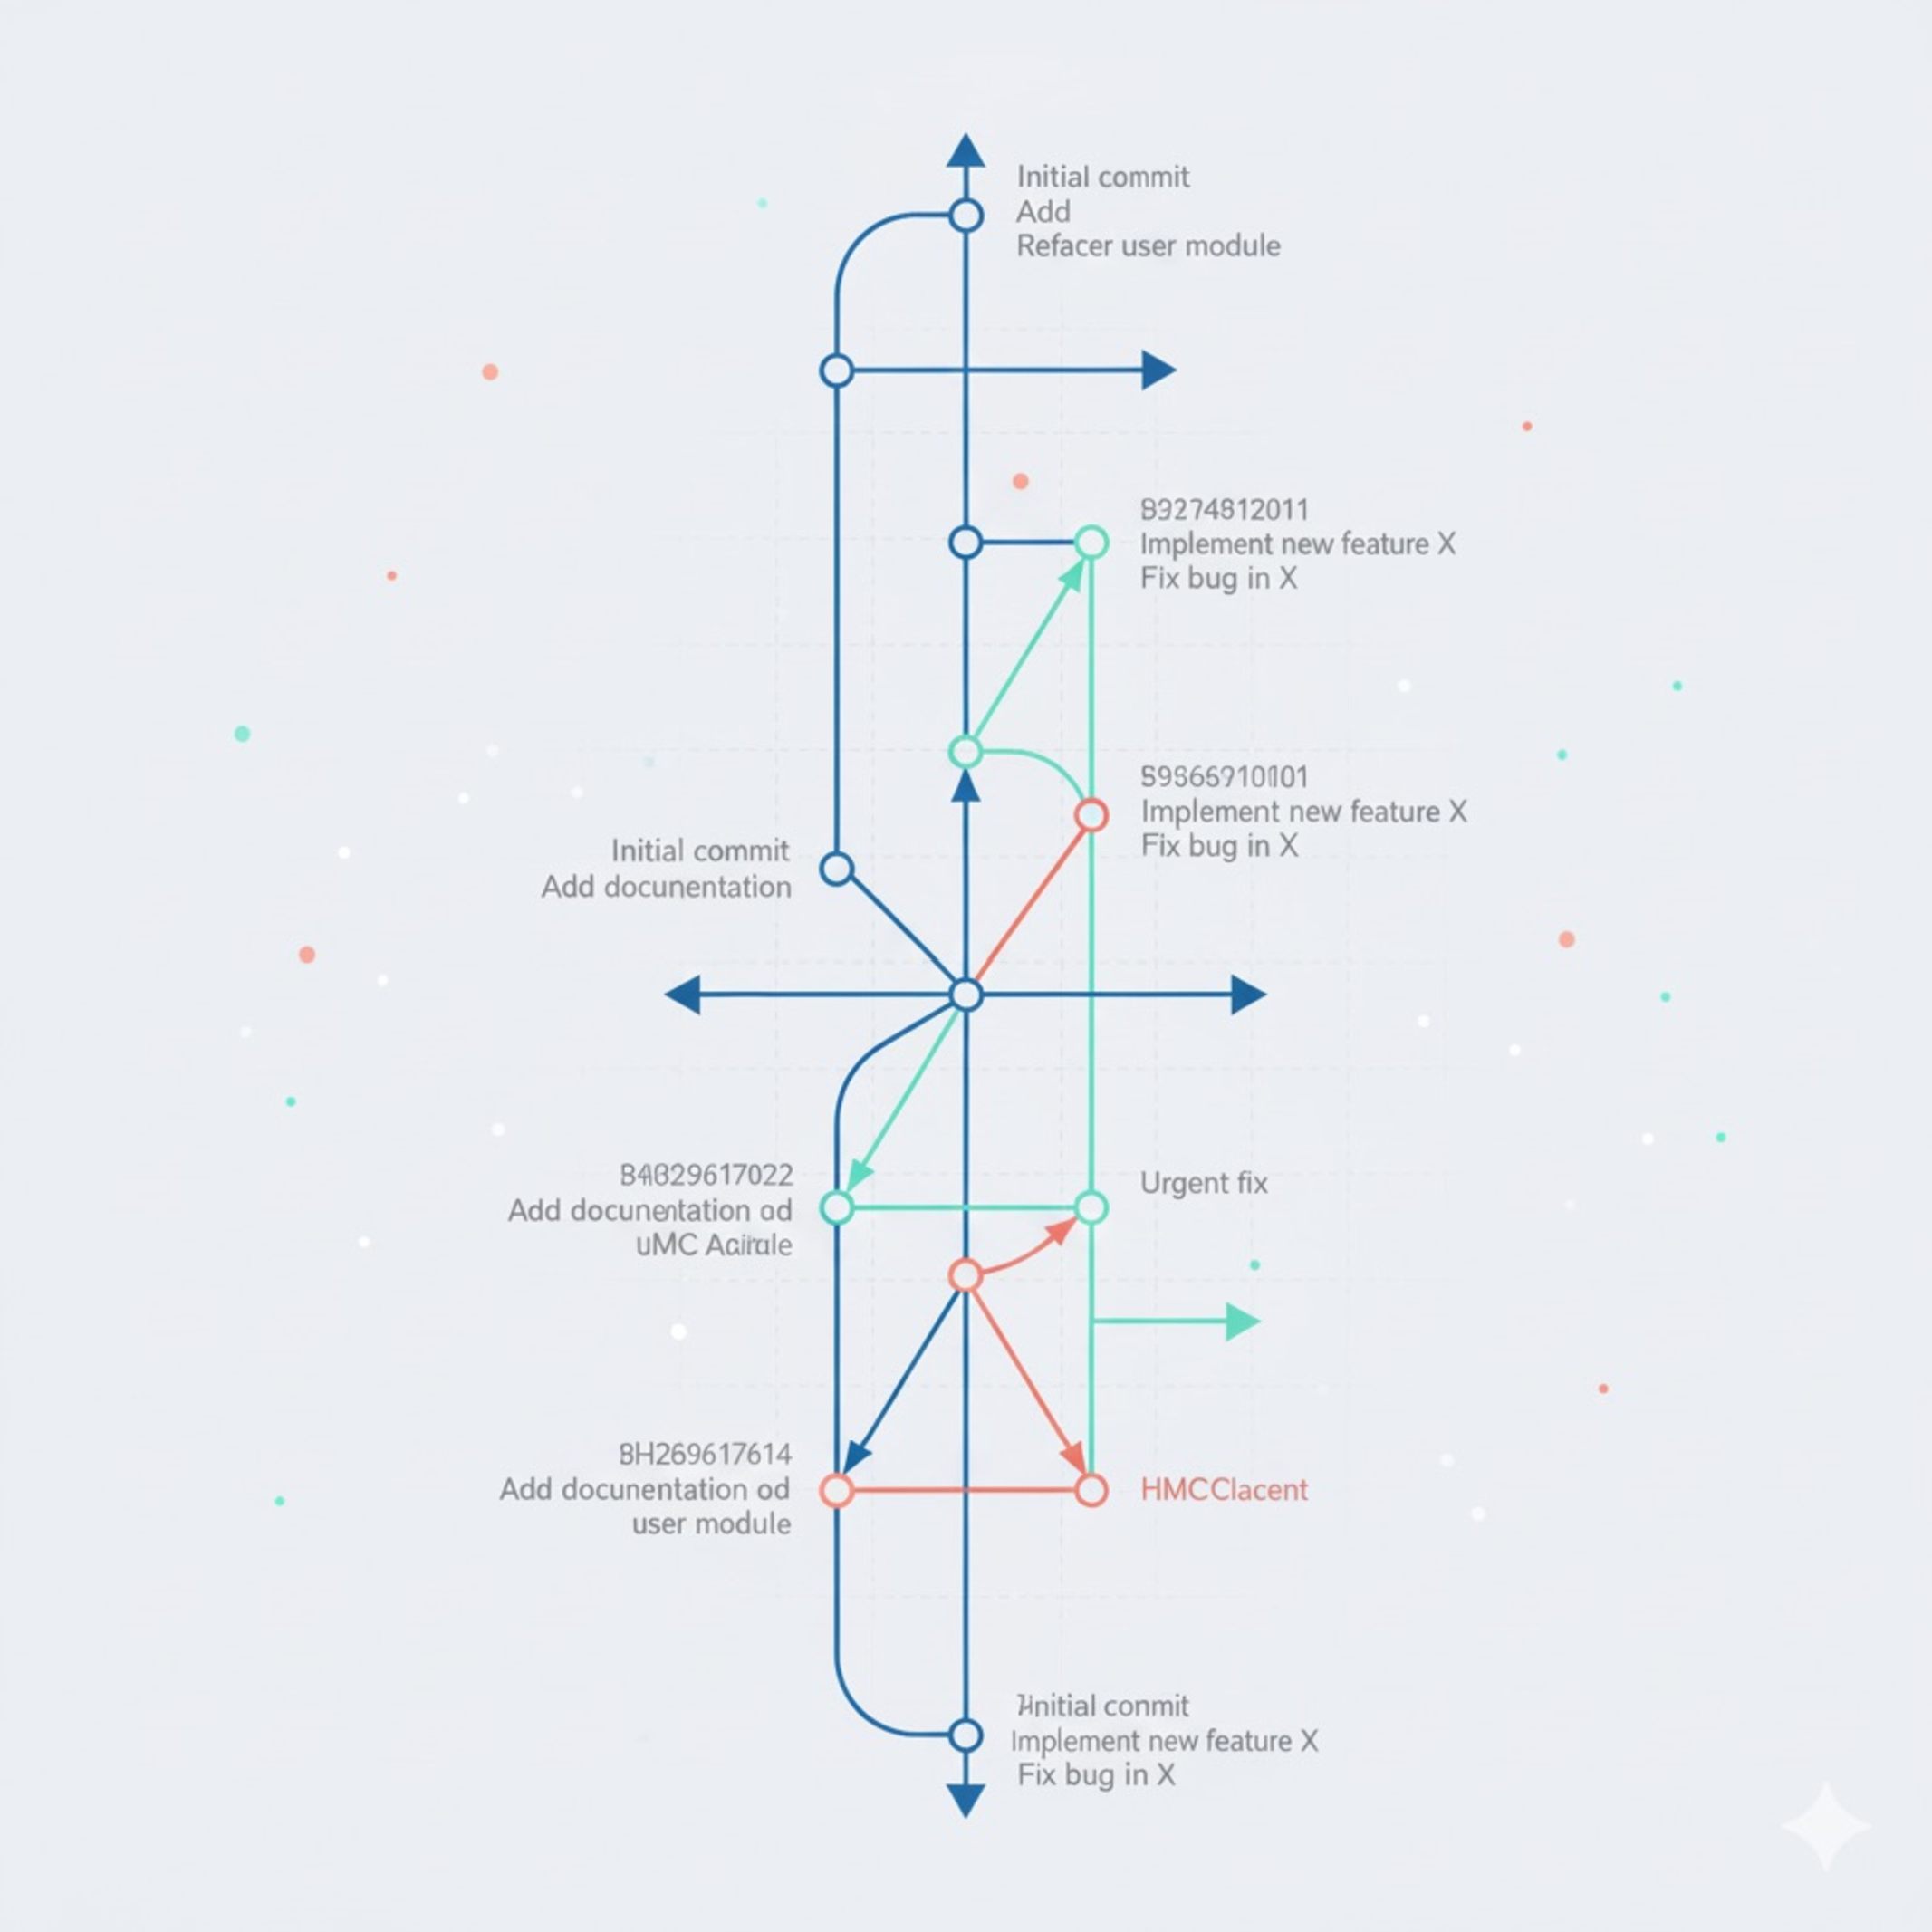
\includegraphics[width=\textwidth]{figs/fig_d1p3/d1p3_01-log}
        \captionof{figure}{Git provides a full history of changes.}
        
        \column{.64\textwidth}
        Your analysis script (e.g., `analyse.py`) is \textbf{data}. It's the recipe that turns raw data into a result. \\
        \pause
        \textbf{Problem:}
        `analyse\_v1.py`
        `analyse\_v2\_final.py`
        `analyse\_v2\_final\_FOR\_REAL.py` \\
        \pause
        This is a \textbf{traceability nightmare}. You no longer know which script made which figure. \\ % This is a \textbf{Data Integrity} failure. \\
        \pause
        \textbf{Solution: Git}
        \begin{itemize}
            \item `git commit -m "Added new filtering step"`
            \item `git commit -m "Fixed bug in axis label"`
        \end{itemize}
        Now you have 100\% traceability.
    \end{columns}
\end{frame}

\begin{frame}{Theory: The Message Broker}{Module 3.3: Configure}
    %% \begin{center}
    %%     \includegraphics[width=0.8\textwidth]{example-image-b}
    %%     \captionof{figure}{A message broker acts as a central post office for data.}
    %% \end{center}
    
    A \textbf{Message Broker} (like Kafka, RabbitMQ, or MQTT) is a tool that routes data streams.
    \pause
    \begin{itemize}
        \item \textbf{Instrument} $\rightarrow$ "Publishes" data to a topic (e.g., `lab/microscope/raw\_data`)
        \pause
        \item \textbf{Broker} $\rightarrow$ Receives the data.
        \pause
        \item \textbf{ELN} $\rightarrow$ "Subscribes" to the topic and automatically ingests the data.
        \item \textbf{Archive} $\rightarrow$ \textit{Also} subscribes and makes a backup.
    \end{itemize}
    \pause
    This is the gold standard for automated, high-integrity data capture.
\end{frame}

\begin{frame}{Interactive: Hands-On Traceability}{Module 3.3: Practice}
    \begin{block}{Workshop (20 min)}
        This is a hands-on session.
    \end{block}
    %% \begin{columns}
    %%     \column{.5\textwidth}
        \begin{block}{Track 1: Version Control (Git)}
            \textbf{Goal:} \textbf{Execute} version control.
            \pause
            \begin{itemize}
                \item Create a folder.
                \item Create `script.py`.
                \item Run: `git init`
                \item Run: `git add .`
                \item Run: `git commit -m "Initial commit"`
            \end{itemize}
            You just ensured traceability!
        \end{block}

       %% \column{.5\textwidth}
       %% \begin{block}{Track 2: Message Broker (Demo)}
       %%     \textbf{Goal:} \textbf{Configure} a broker.
       %%     \pause
       %%     \begin{itemize}
       %%         \item (Live Demo)
       %%         \item 1. Start a simple MQTT broker.
       %%         \item 2. Run a "sensor" script that publishes data.
       %%         \item 3. Run a "logger" script that subscribes and prints the data.
       %%     \end{itemize}
       %% \end{block}
    %% \end{columns}
\end{frame}

\begin{frame}{Learning Objectives (3.4)}
    \begin{itemize}
        \item \textbf{Differentiate} between data annotation methods for \emph{qualitative} vs. \emph{quantitative} data.
        \item \textbf{Troubleshoot} a data pipeline error by \textbf{analysing} message broker logs.
    \end{itemize}
\end{frame}

\begin{frame}{Theory: Data Annotation Methods}{Module 3.4: Differentiate}
    Annotation (metadata) is not one-size-fits-all.
    
    \begin{columns}
        \column{.5\textwidth}
        \begin{block}{Quantitative Data (Numbers)}
            \textbf{Data:} `10.5`
            \textbf{Annotation Needs:}
            \begin{itemize}
                \item \textbf{Vocabularies:} What is it? (e.g., `PATO:0000125` - "temperature" see \href{https://www.ebi.ac.uk/ols4/}{OLS})
                \item \textbf{Units:} What unit? (e.g., `UO:0000027` - "degree Celsius")
                \item \textbf{Precision:} `+/- 0.05`
            \end{itemize}
            \textbf{Goal:} Consistency, machine-readability.
        \end{block}
        
        \column{.5\textwidth}
        \begin{block}{Qualitative Data (Text/Image)}
            \textbf{Data:} "The sample showed significant degradation..."
            \textbf{Annotation Needs:}
            \begin{itemize}
                \item \textbf{Coding Schemas:} What does "significant degradation" mean? (e.g., `Degradation\_Level\_3`)
                \item \textbf{Context:} Who wrote this? When?
                \item \textbf{Tags:} `\#failed\_experiment`, `\#contamination`
            \end{itemize}
            \textbf{Goal:} Context, findability, interpretation.
        \end{block}
    \end{columns}
\end{frame}

\begin{frame}{Theory: Troubleshooting the Pipeline}{Module 3.4: Troubleshoot}
    %% \begin{center}
    %%     \includegraphics[width=0.7\textwidth]{example-image-a}
    %%     \captionof{figure}{Instrument $\rightarrow$ Broker $\rightarrow$ ELN}
    %% \end{center}
    
    \textbf{Problem:} The ELN is recording gibberish, but the instrument seems fine. Where is the error?
    \pause
    \begin{itemize}
        \item \textbf{Step 1:} Check the Message Broker logs. Is the data arriving at the broker correctly?
        \pause
        \item \textbf{Yes:} The data is fine. The problem is the \textbf{ELN subscriber} (Track 2). It's misinterpreting the message.
        \pause
        \item \textbf{No:} The data is not in the logs, or it's already gibberish. The problem is the \textbf{Instrument publisher} (Track 1). It's sending bad data.
    \end{itemize}
    \pause
    The broker's log is your central point for \textbf{troubleshooting}.
\end{frame}

\begin{frame}{Interactive: The Pipeline is Broken!}{Module 3.4: Practice}
    \begin{block}{Scenario (15 min)}
        \textbf{Problem:} Your ELN is recording temperatures as `25.3` (correct), but pressures as `NULL`.
        \pause
        \textbf{Logs:} The broker log shows:
        `{"topic": "lab/sensor/temp", "payload": "25.3"}`
        `{"topic": "lab/sensor/pressure", "payload": "101.3"}`
        \pause
        \textbf{Task: Analyse \& Troubleshoot}
        \begin{itemize}
            \item Is the instrument working? (Yes)
            \item Is the broker working? (Yes)
            \item What is the problem?
            \pause
            \item \textbf{Answer:} The ELN is subscribed to `lab/sensor/temp` but \emph{not} to `lab/sensor/pressure`. It's a configuration error in the subscriber.
        \end{itemize}
        \textbf{Goal:} \textbf{Troubleshoot} a pipeline error.
    \end{block}
\end{frame}

\begin{frame}{Learning Objectives (3.5)}
    \begin{itemize}
        \item \textbf{Assess} the current team workflow against the DMP.
        \item \textbf{Compare} and \textbf{evaluate} manual vs. automated data capture, justifying the superior method based on \textbf{verifiability}.
    \end{itemize}
\end{frame}

\begin{frame}{Theory: Assessing Workflow vs. DMP}{Module 3.5: Assess}
    Your DMP is your \textbf{plan}. Your workflow is your \textbf{reality}. You must \textbf{assess} reality against the plan. \\
    \pause
    \begin{block}{The "DMP Audit"}
        \textbf{Your DMP says:} "All data will be annotated with a standard vocabulary." \\
        \pause
        \textbf{Your Workflow is:} A student is typing free-text notes into the ELN. \\
        \pause
        \textbf{Result:} \textbf{Non-compliant.} You have a bottleneck. \\
        \pause
        \textbf{Solution:} You must \textbf{assess} this gap and fix it (e.g., build a drop-down list in the ELN). \\
    \end{block}
\end{frame}

\begin{frame}{Theory: Manual vs. Automated (Verifiability)}{Module 3.5: Compare}
    \textbf{Verifiability} (Data Integrity) is the ability to prove your data is correct.
    
    \begin{columns}
        \column{.5\textwidth}
        \begin{block}{Method 1: Manual Entry}
            \begin{itemize}
                \item Student reads "10.5" from screen.
                \item Student types "10.5" into Excel.
                \item \textbf{Verifiability:} Low.
                \item \textbf{Error Points:} Typo? Did they misread? Did they skip a line? You can \emph{never} be 100\% sure.
            \end{itemize}
        \end{block}
        
        \column{.5\textwidth}
        \begin{block}{Method 2: Automated Pipeline}
            \begin{itemize}
                \item Instrument sends "10.5".
                \item Broker logs "10.5".
                \item ELN records "10.5".
                \item \textbf{Verifiability:} High.
                \item \textbf{Error Points:} None (in transcription). The log \emph{proves} what the instrument sent.
            \end{itemize}
        \end{block}
    \end{columns}
    \pause
    \textbf{Justification:} The automated pipeline is superior not because it's faster, but because it is \textbf{verifiable}.
\end{frame}

\begin{frame}{Interactive: Debate - Manual vs. Automated}{Module 3.5: Practice}
    \begin{block}{Group Evaluation (10 min)}
        \textbf{Scenario:} A senior professor says, "These new automated pipelines are a black box. I trust my PhD students to write down the numbers correctly. It's how I've always done it."
        \pause
        \textbf{Task:}
        \begin{itemize}
            \item \textbf{Compare} the two methods.
            \item Form a polite, respectful argument. \textbf{Justify} why the automated pipeline is superior, using the concept of \textbf{verifiability}.
        \end{itemize}
        \pause
        \textbf{Goal:} \textbf{Evaluate} two methods.
    \end{block}
\end{frame}

\begin{frame}{Learning Objectives (3.6)}
    \begin{itemize}
        \item \textbf{Develop} a comprehensive, step-by-step \textbf{workflow diagram} that integrates automated metadata creation.
        \item \textbf{Design} a resilient, end-to-end RDM workflow for data collection.
    \end{itemize}
\end{frame}


\begin{frame}{Theory: The End-to-End Workflow}
    
    \begin{itemize}
        \item \textbf{Plan:} DMP (from RDMO)
        \item \textbf{Acquire:} Instrument + Instrument Registry
        \item \textbf{Transport:} Message Broker
        \item \textbf{Record:} ELN (with required fields)
        \item \textbf{Process:} Analysis Scripts (versioned in Git)
        \item \textbf{Publish:} Repository (KITOpen / OEP)
    \end{itemize}
\end{frame}


\begin{frame}{Theory: The End-to-End Workflow}{Module 3.6: Develop}
    Let's put all the pieces from today together.
    \begin{center}
        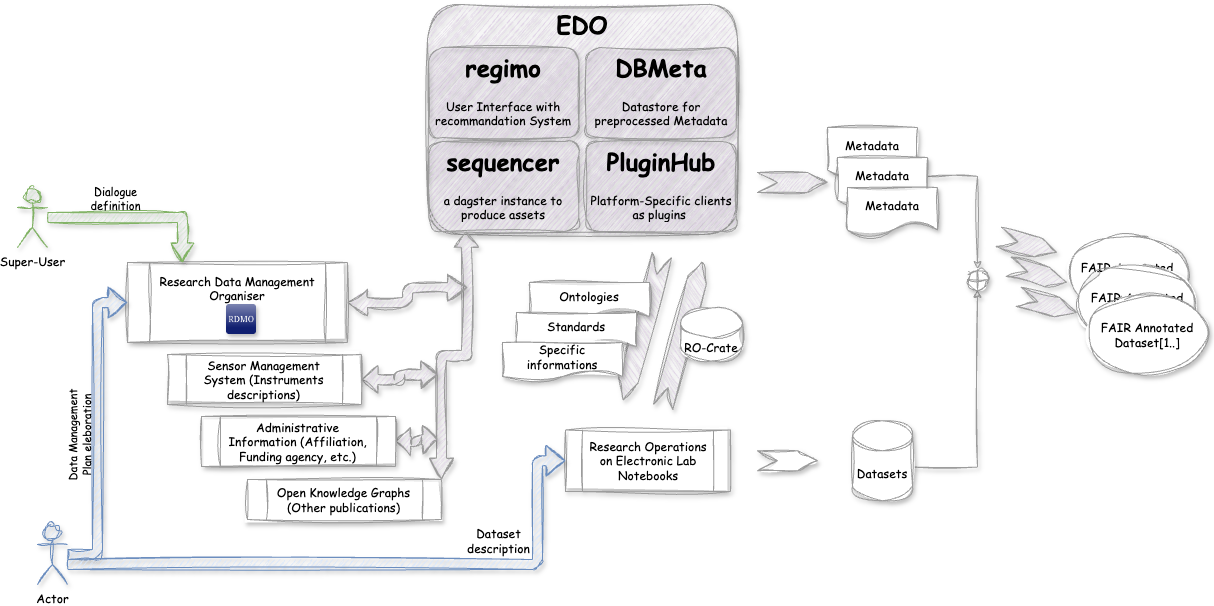
\includegraphics[width=.72\textwidth]{figs/fig_d1p3/edo_overview.png}
        \captionof{figure}{A conceptual diagram of a full RDM-integrated workflow.}
    \end{center}
\end{frame}

\begin{frame}{Interactive: Design Your Workflow}{Module 3.6: Practice}
    \begin{block}{Activity: Whiteboard Session (20 min)}
        \textbf{Task:} As a group, \textbf{design} your ideal, resilient, end-to-end RDM workflow.
        \pause
        \textbf{Instructions:}
        \begin{itemize}
            \item Draw it on a whiteboard or paper.
            \item Start with the \textbf{Instrument}.
            \item End with the \textbf{Publication} (on KITOpen/OEP).
            \item \textbf{Must Include:} Your ELN, a Message Broker, and Git.
            \item Show where metadata is created and where it flows.
        \end{itemize}
        \pause
        \textbf{Goal:} \textbf{Develop} and \textbf{Design} a comprehensive workflow diagram.
    \end{block}
\end{frame}

\begin{frame}{Module 3: Summary}
    \begin{itemize}
        \item RDM is not just planning; it's \textbf{daily operation}.
        \item \textbf{ELNs} are the core tool for capturing metadata at acquisition.
        \item \textbf{Git} ensures traceability (integrity) for your scripts.
        \item \textbf{Message Brokers} provide a verifiable, automated path from instrument to ELN.
        \item We must \textbf{assess} our real workflow against our DMP.
    \end{itemize}
    \vfill
    \begin{center}
        \textbf{End of Day 1}
    \end{center}
\end{frame}